
%(BEGIN_QUESTION)
% Copyright 2006, Tony R. Kuphaldt, released under the Creative Commons Attribution License (v 1.0)
% This means you may do almost anything with this work of mine, so long as you give me proper credit

Purge-systemer kan brukes til å måle hydrostatisk trykk i en tank selv uten dypperør.  I dette nivåmålesystemet brukes trykkluft som purge-medium direkte inn i tanken der transmitterrørene er koblet:

$$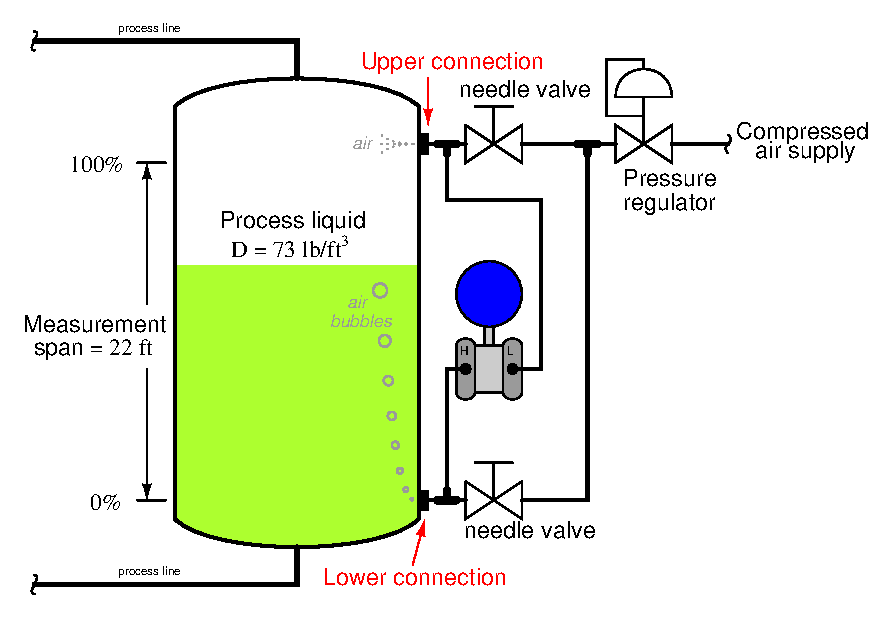
\includegraphics[width=15.5cm]{i00250x01.eps}$$

Beregn først riktig kalibreringsområde for DP-transmitteren i denne applikasjonen.

\vskip 10pt

Forklar deretter hva som skjer med transmitterutgangen hvis den nedre prosessforbindelsen til tanken tettes av avleiringer (til tross for renseeffekten fra komprimert luft som strømmer gjennom).  Alternativt: hva hvis bare den øvre forbindelsen tettes?

\vskip 20pt \vbox{\hrule \hbox{\strut \vrule{} {\bf Forslag til sokratisk diskusjon} \vrule} \hrule}

\begin{itemize}
\item{} Hvorfor velger noen å kontinuerlig \textit{purge} tilkoblingene på en hydrostatisk nivåtransmitter når de kunne brukt fjernforseglinger (membraner)?
\item{} Er luft alltid et trygt purge-medium?  Hvis ikke, hva er gyldige alternativer?
\item{} Anta at en propp av prosessvæske kommer inn i impulsledningen på ``H''-siden til DP-transmitteren.  Hvordan påvirker dette nøyaktigheten?
\item{} Anta at en propp av prosessvæske kommer inn i impulsledningen på ``L''-siden til DP-transmitteren.  Hvordan påvirker dette nøyaktigheten?
\end{itemize}

\underbar{file i00250}
%(END_QUESTION)





%(BEGIN_ANSWER)

Hvis den nedre prosessforbindelsen blokkeres av avleiringer, vil transmitterens utgangssignal øke, muligens til mer enn 100\%.  Det motsatte skjer hvis den øvre prosessforbindelsen blokkeres.

%(END_ANSWER)





%(BEGIN_NOTES)

DP-område = 0 til 308.8 "W.C = 0 til 11.15 PSID

\vskip 10pt

Hvis den nedre prosessforbindelsen blokkeres av avleiringer, vil transmitterens utgangssignal øke, muligens til mer enn 100\%.  Det motsatte skjer hvis den øvre prosessforbindelsen blokkeres.

%INDEX% Measurement, level: hydrostatic pressure (purged)

%(END_NOTES)
